% 2013 辽宁卷文科第 18 题：PA 垂直圆面，C 在圆上，Q 为 PA 中点，G 为 △AOC 重心。
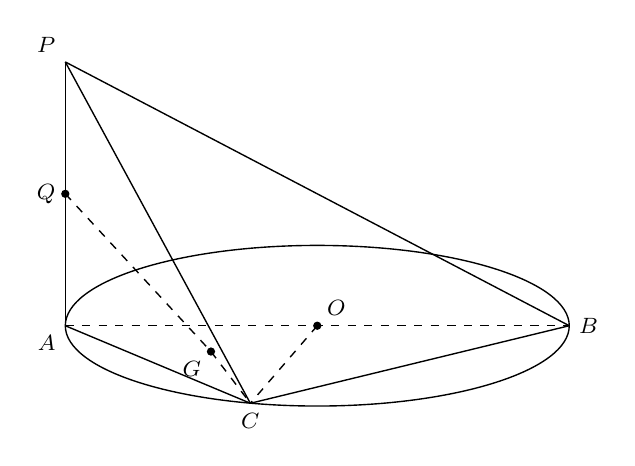
\begin{tikzpicture}[font=\footnotesize, line width=0.5pt, scale=1]
  \coordinate (O) at (0,0);
  \coordinate (A) at (-3.2,0);
  \coordinate (B) at (3.2,0);
  \coordinate (C) at (-0.85,-0.985);
  \coordinate (P) at (-3.2,3.35);
  \coordinate (Q) at (-3.2,1.675);
  \coordinate (G) at (-1.35,-0.328);
  % 底面圆（斜二测画法下的椭圆）
  \draw (0,0) ellipse (3.2 and 1.02);
  % 可见棱
  \draw (P) -- (A);
  \draw (P) -- (B);
  \draw (P) -- (C);
  \draw (A) -- (C);
  \draw (C) -- (B);
  % 被遮挡的线
  \draw[dashed] (A) -- (B);
  \draw[dashed] (O) -- (C);
  \draw[dashed] (Q) -- (G);
  \draw[dashed] (G) -- (C);
  % 点与标签
  \fill (O) circle (1.5pt) node[above right] {$O$};
  \fill (Q) circle (1.5pt) node[left] {$Q$};
  \fill (G) circle (1.5pt) node[below left] {$G$};
  \node[above left] at (P) {$P$};
  \node[below left] at (A) {$A$};
  \node[right] at (B) {$B$};
  \node[below] at (C) {$C$};
\end{tikzpicture}
